\section{Introduction}
Notation of western classical music has used a combination of the diastematic and phonetic notation \parencite{RRastall} since the advent of Gregorian chant around 640AD \parencite{RTaruskin}. The function of this notation falls into two main divisions: the expression of relationship in sound frequency, and the expression of relationship in time, or measure \parencite{oxHistory}.

The key element of this form of notation is the staff, as shown in Figure 1 below. This is a grouping of five horizontal lines, with each line or space in the staff indicating a different sound pitch, a term meaning the relative "highness" or "lowness" of the sound \parencite{classroom}.

\begin{figure}[htbp]
    \centering
        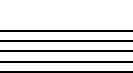
\includegraphics{staff-crop.pdf}
    \caption{A blank staff}
\end{figure}

This staff is divided by barlines, vertical lines delineating grouped units of sound and silence (formally referred to as notes and rests), which provides an indication of the unit's relationship in time by its juxtaposition to other groupings in the composition. These groupings are called measures or bars, with each bar having a variable maximum of notes and rests. 

\begin{figure}[htbp]
    \centering
        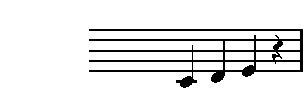
\includegraphics{bar_with_notes-crop.pdf}
    \caption{A bar containing three notes and one rest}
\end{figure}

The representations of other parameters in staff notation are normally phonetic, such as indications p - meaning piano, or "quiet" - and pizz - meaning pizzicato, or "plucked" \parencite{RRastall}. This mechanism is complex in nature, and has a large but finite set of symbols which control every element of the composition.

A musician will often organise pieces notated using this system, or scores as they are formally known, in a music cabinet or filing cabinet \parencite{musicOrganising}. These range from basic shelving to the more traditional large ornate cabinets where drawers only allow the user to see the top document, making it difficult to find scores which are deeper in the cabinet. This can often mean that music a performer will use regularly is kept on music stands and in piano stools, because if they were to return an item back into the music cabinet, it is likely that they would never find it again \parencite{SheetMusicRant}.

This makes it difficult for instrumentalists to find a good way to organise their collections - this particular physical method allows for only one or two ordering choices, whereas the described notation system has many ways in which a piece can be identified. 

It would be useful to a variety of musicians to be able to organise and search their collections using more than one mechanism. Such mechanisms have been developed in software automatically to cater for song title and composer name, but only allow for more detailed organisation by asking the user to provide more complex meta information \parencite{calypso}. In a physical system this type of organisation would require file duplication. This project aims to create a sheet music organisation system for virtual music organisation, which will provide an automatic mechanism for the described problem.

This document discusses the aims and objectives of this project, background setting the project in a technical perspective, designs for the development of the solution, and a review of progress and project management to date. 
\pagebreak
\section{Aims and Objectives}
\subsection{Project Aim}
\begin{center}
\textit{The overall aim of the project is to design and develop a sheet music library application, with the ability to organise and view personal sheet music collections, and download sheet music from the internet. Time permitting, it should also be able to generate sound from the sheet music, and import editable music from flat images.}
\end{center}
\subsection{Primary Objectives}
The following objectives are of the highest importance to the project, and are a measure of whether the project has been completed.
\begin{itemize}
    \item \textbf{Rendering of Musical Files}\\
    It will be necessary to render one or more formats of commonly stored musical files, as the aim of the project is to enable users to view and organise their sheet music collections.
    \item \textbf{Extraction of Metadata}\\
    The project will be required to extract important information from each piece, ranging from the simple nominal data such as title, composer, lyricist, to the more complex notation such as clefs, key signatures and meters used. 
    \item \textbf{Connection to Online Music Collections}\\
    It should also be possible to connect to online music collections, as it would be beneficial to users to be able to search and add to their collections using the same interface.

\end{itemize}
\subsection{Secondary Objectives}
The following objectives are to be completed if the primary objectives are met, and as such do not dictate the success or failure of the project, but rather are features which would add value.

\begin{itemize}
    \item \textbf{Audio playback}\\
    It would be useful to a cross section of users to be able to play music files as sound clips. This enables performers who regularly play with an accompaniest or ensemble to create practice accompaniments from their sheet music, or hear an approximation of how a melody should sound.
    \item \textbf{MusicOCR conversion of images to parseable MusicXML}\\
It would be easier for musicians to merge their physical and virtual music collections for automatic organisation if the solution provided a way to import flat, scanned sheet music into knowledgeable music files. 
\end{itemize}
